\documentclass{standalone}
\usepackage{libertinus}
\usepackage{tikz}

\begin{document}

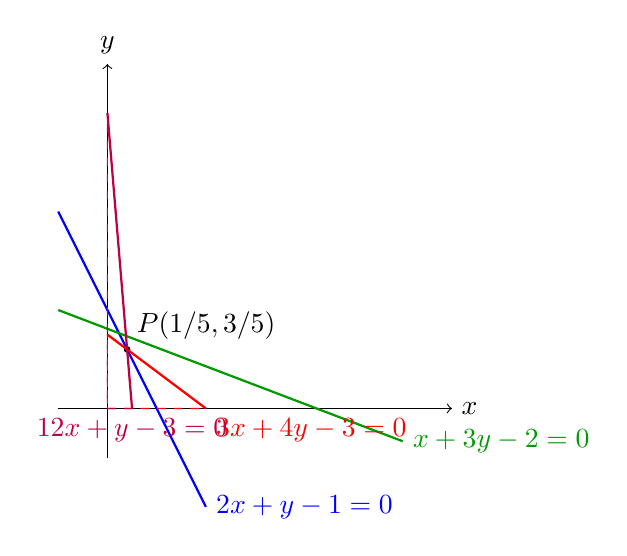
\begin{tikzpicture}[x=1.25cm, y=1.25cm]

% Axes
\draw[->] (-0.5,0) -- (3.5,0) node[right] {$x$};
\draw[->] (0,-0.5) -- (0,3.5) node[above] {$y$};

% Given lines
\draw[blue, thick] (-0.5,2) -- (1,-1) node[right] {$2x + y - 1 = 0$};
\draw[green!60!black, thick] (-0.5,1) -- (3,-1/3) node[right] {$x + 3y - 2 = 0$};

% Intersection point
\filldraw (1/5,3/5) circle (1pt) node[above right] {$P(1/5, 3/5)$};

% First required line: 3x + 4y - 3 = 0
\draw[red, thick] (0,3/4) -- (1,0) node[below right] {$3x + 4y - 3 = 0$};

% Triangle 1
\draw[dashed, red] (0,0) -- (1,0) -- (0,3/4) -- cycle;

% Second required line: 12x + y - 3 = 0
\draw[purple, thick] (0,3) -- (1/4,0) node[below] {$12x + y - 3 = 0$};

% Triangle 2
\draw[dashed, purple] (0,0) -- (1/4,0) -- (0,3) -- cycle;

\end{tikzpicture}

\end{document}
